% Author: Jørn Olav Jensen

\newpage
\section{Suggested solutions: Ideal and Tapered Filters}

\begin{marginfigure}
  \begin{center}
    \begin{tikzpicture}
      \begin{axis}[width=7cm,height=6cm,ymin=0,xmin=-3.0,ymax=1.5,xmax=3.0,  yticklabels={,,},
          xtick={-2.5,-1.5,-0.5,0.5,1.5,2.5},
          xticklabels={$-\pi$,$-\omega_1$,$-\omega_0$,$\omega_0$,$\omega_1$,$\pi$},
          ylabel=$\He$,
          xlabel=$\hat{\omega}$, axis lines = center]

        \addplot[mark=none,color=blue] coordinates {
            (-2.5,1)
            (-1.5,1)
            (-1.5,0)
            (-0.5,0)
            (-0.5,1)
            (0.5,1)
            (0.5,0)
            (1.5,0)
            (1.5,1)
            (2.5,1)
          };
      \end{axis}
    \end{tikzpicture}
  \end{center}
  \caption{The frequency response of an ideal stop-pass filter.}
  \label{fig:ideal_bs_fr}
\end{marginfigure}

\begin{enumerate}
  % Exercise 1
  \item Let the ideal band-stop filter be given as:
        \begin{equation*}
          \mathcal{H}_{\mathrm{BS}}(\hat{\omega}) = \left\{ \begin{array}{cc}
            0 & \hat{\omega}_0 < |\hat{\omega}| < \hat{\omega}_1 \\
            1 & \mathrm{otherwise}
          \end{array}\right.\,\,.
        \end{equation*}
        The impulse response can then be computed using the inverse DTFT as follows (see Figure \ref{fig:ideal_bs_fr}):
        \begin{align*}
          h[n] & =\frac{1}{2\pi}\int_{-\pi}^{\pi}\mathcal{H}_{\mathrm{BS}}(\hat{\omega})e^{i\hat{\omega}n}d\hat{\omega},                                                                                                                                                                        \\
               & =\frac{1}{2\pi}\int_{-\pi}^{-\hat{\omega}_{1}}e^{i\hat{\omega}n}d\hat{\omega} + \frac{1}{2\pi}\int_{-\hat{\omega}_{0}}^{\hat{\omega}_{0}}e^{i\hat{\omega}n}d\hat{\omega} + \frac{1}{2\pi}\int_{\hat{\omega}_{1}}^{\pi}e^{i\hat{\omega}n}d\hat{\omega},                         \\
               & =\frac{1}{2\pi}\left[\frac{1}{in}e^{i\hat{\omega}n}\right]_{-\pi}^{-\hat{\omega}_{1}} + \frac{1}{2\pi}\left[\frac{1}{in}e^{i\hat{\omega}n}\right]_{-\hat{\omega}_{0}}^{\hat{\omega}_{0}} + \frac{1}{2\pi}\left[\frac{1}{in}e^{i\hat{\omega}n}\right]_{\hat{\omega}_{1}}^{\pi}, \\
               & =\frac{1}{2in\pi}\left(e^{-i\hat{\omega}_{1}n}-e^{-i\pi n}\right) + \frac{1}{2in\pi}\left(e^{i\hat{\omega}_{0}n}-e^{-i\hat{\omega}_{0}n}\right) + \frac{1}{2in\pi}\left(e^{i\pi n}-e^{i\hat{\omega}_{1}n}\right),                                                              \\
               & =\frac{1}{n\pi}\sin(\pi n) + \frac{1}{n\pi}\sin(\hat{\omega}_{0}n) - \frac{1}{n\pi}\sin(\hat{\omega}_{1}n),                                                                                                                                                                    \\
               & =\delta[n] + \frac{\sin(\hat{\omega}_{0}n)}{n\pi} - \frac{\sin(\hat{\omega}_{1}n)}{n\pi}.
        \end{align*}
        As expected, the ideal stop-pass is just the opposite of an ideal band-pass filter.

  % Exercise 2
  \item Continuing with the filter in the previous exercise.

        \begin{enumerate}[a)]
          % Exercise 2a)
          \item The impulse response of the band-stop filter was shown in the previous exercise to be:
                \[ h[n] = \delta[n] + \frac{\sin(\hat{\omega}_{0}n)}{n\pi} - \frac{\sin(\hat{\omega}_{1}n)}{n\pi}. \]
                A tapered version of this filter is then found by:
                \[ h_{w}[n] = w(n)h[n - N/2], \]
                where $N$ is the length of the filter and the window function. Putting all of this together, we obtain:
                \[ h_{w}[n] = \delta[n-N/2]w[n] + \frac{\sin(\hat{\omega}_{0}(n-N/2))}{(n-N/2)\pi}w[n] - \frac{\sin(\hat{\omega}_{1}(n-N/2))}{(n-N/2)\pi}w[n]. \]

          % Exercise 2b)
          \item An implementation of the band-stop filter is shown in Listing \ref{solex13_2}.

                \lstinputlisting[language=Python, caption=Band-stop filter, label=solex13_2, linerange={0-50}]{ch13/code/ex13_2.py}
                \begin{marginfigure}
                  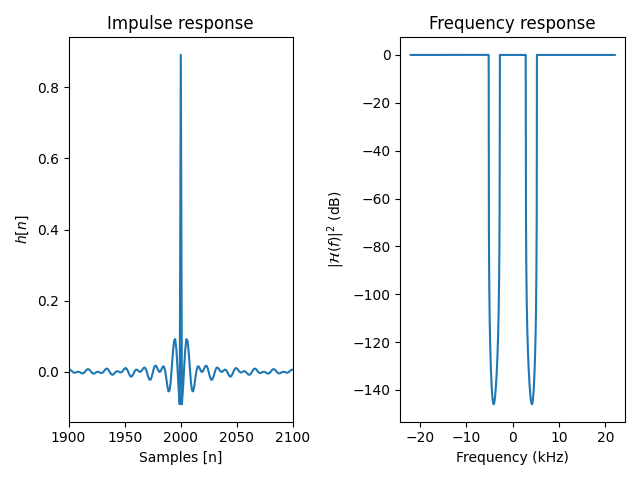
\includegraphics[width=7.0cm, height=6.8cm]{ch13/figures/impulse_response.png}
                  \caption{Impulse response for the band-stop filter}
                  \label{impulse_stop}
                \end{marginfigure}

                In Figure \ref{impulse_stop} a plot of the impulse response for the band-stop filter is shown, both in time and frequency domain.
                In time domain we see the Dirac delta in the middle and also the sinc function behavior.
                For the frequency domain plot the filter is close to what we would expect. Figure \ref{freq_spec_filter} shows that the
                frequency components corresponding to the band between $f_{0}$ and $f_{1}$ have been
                reduced in power. This is what one would except from a band-stop filter.

                \begin{marginfigure}
                  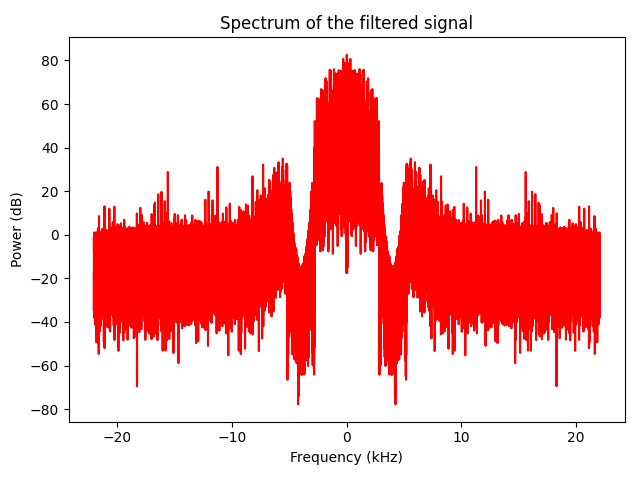
\includegraphics[width=7.0cm, height=7.0cm]{ch13/figures/freq_spec_filter.png}
                  \caption{Frequency spectrum of the filtered signal}
                  \label{freq_spec_filter}
                \end{marginfigure}

        \end{enumerate}
\end{enumerate}